\begin{figure}[h!]
\centering
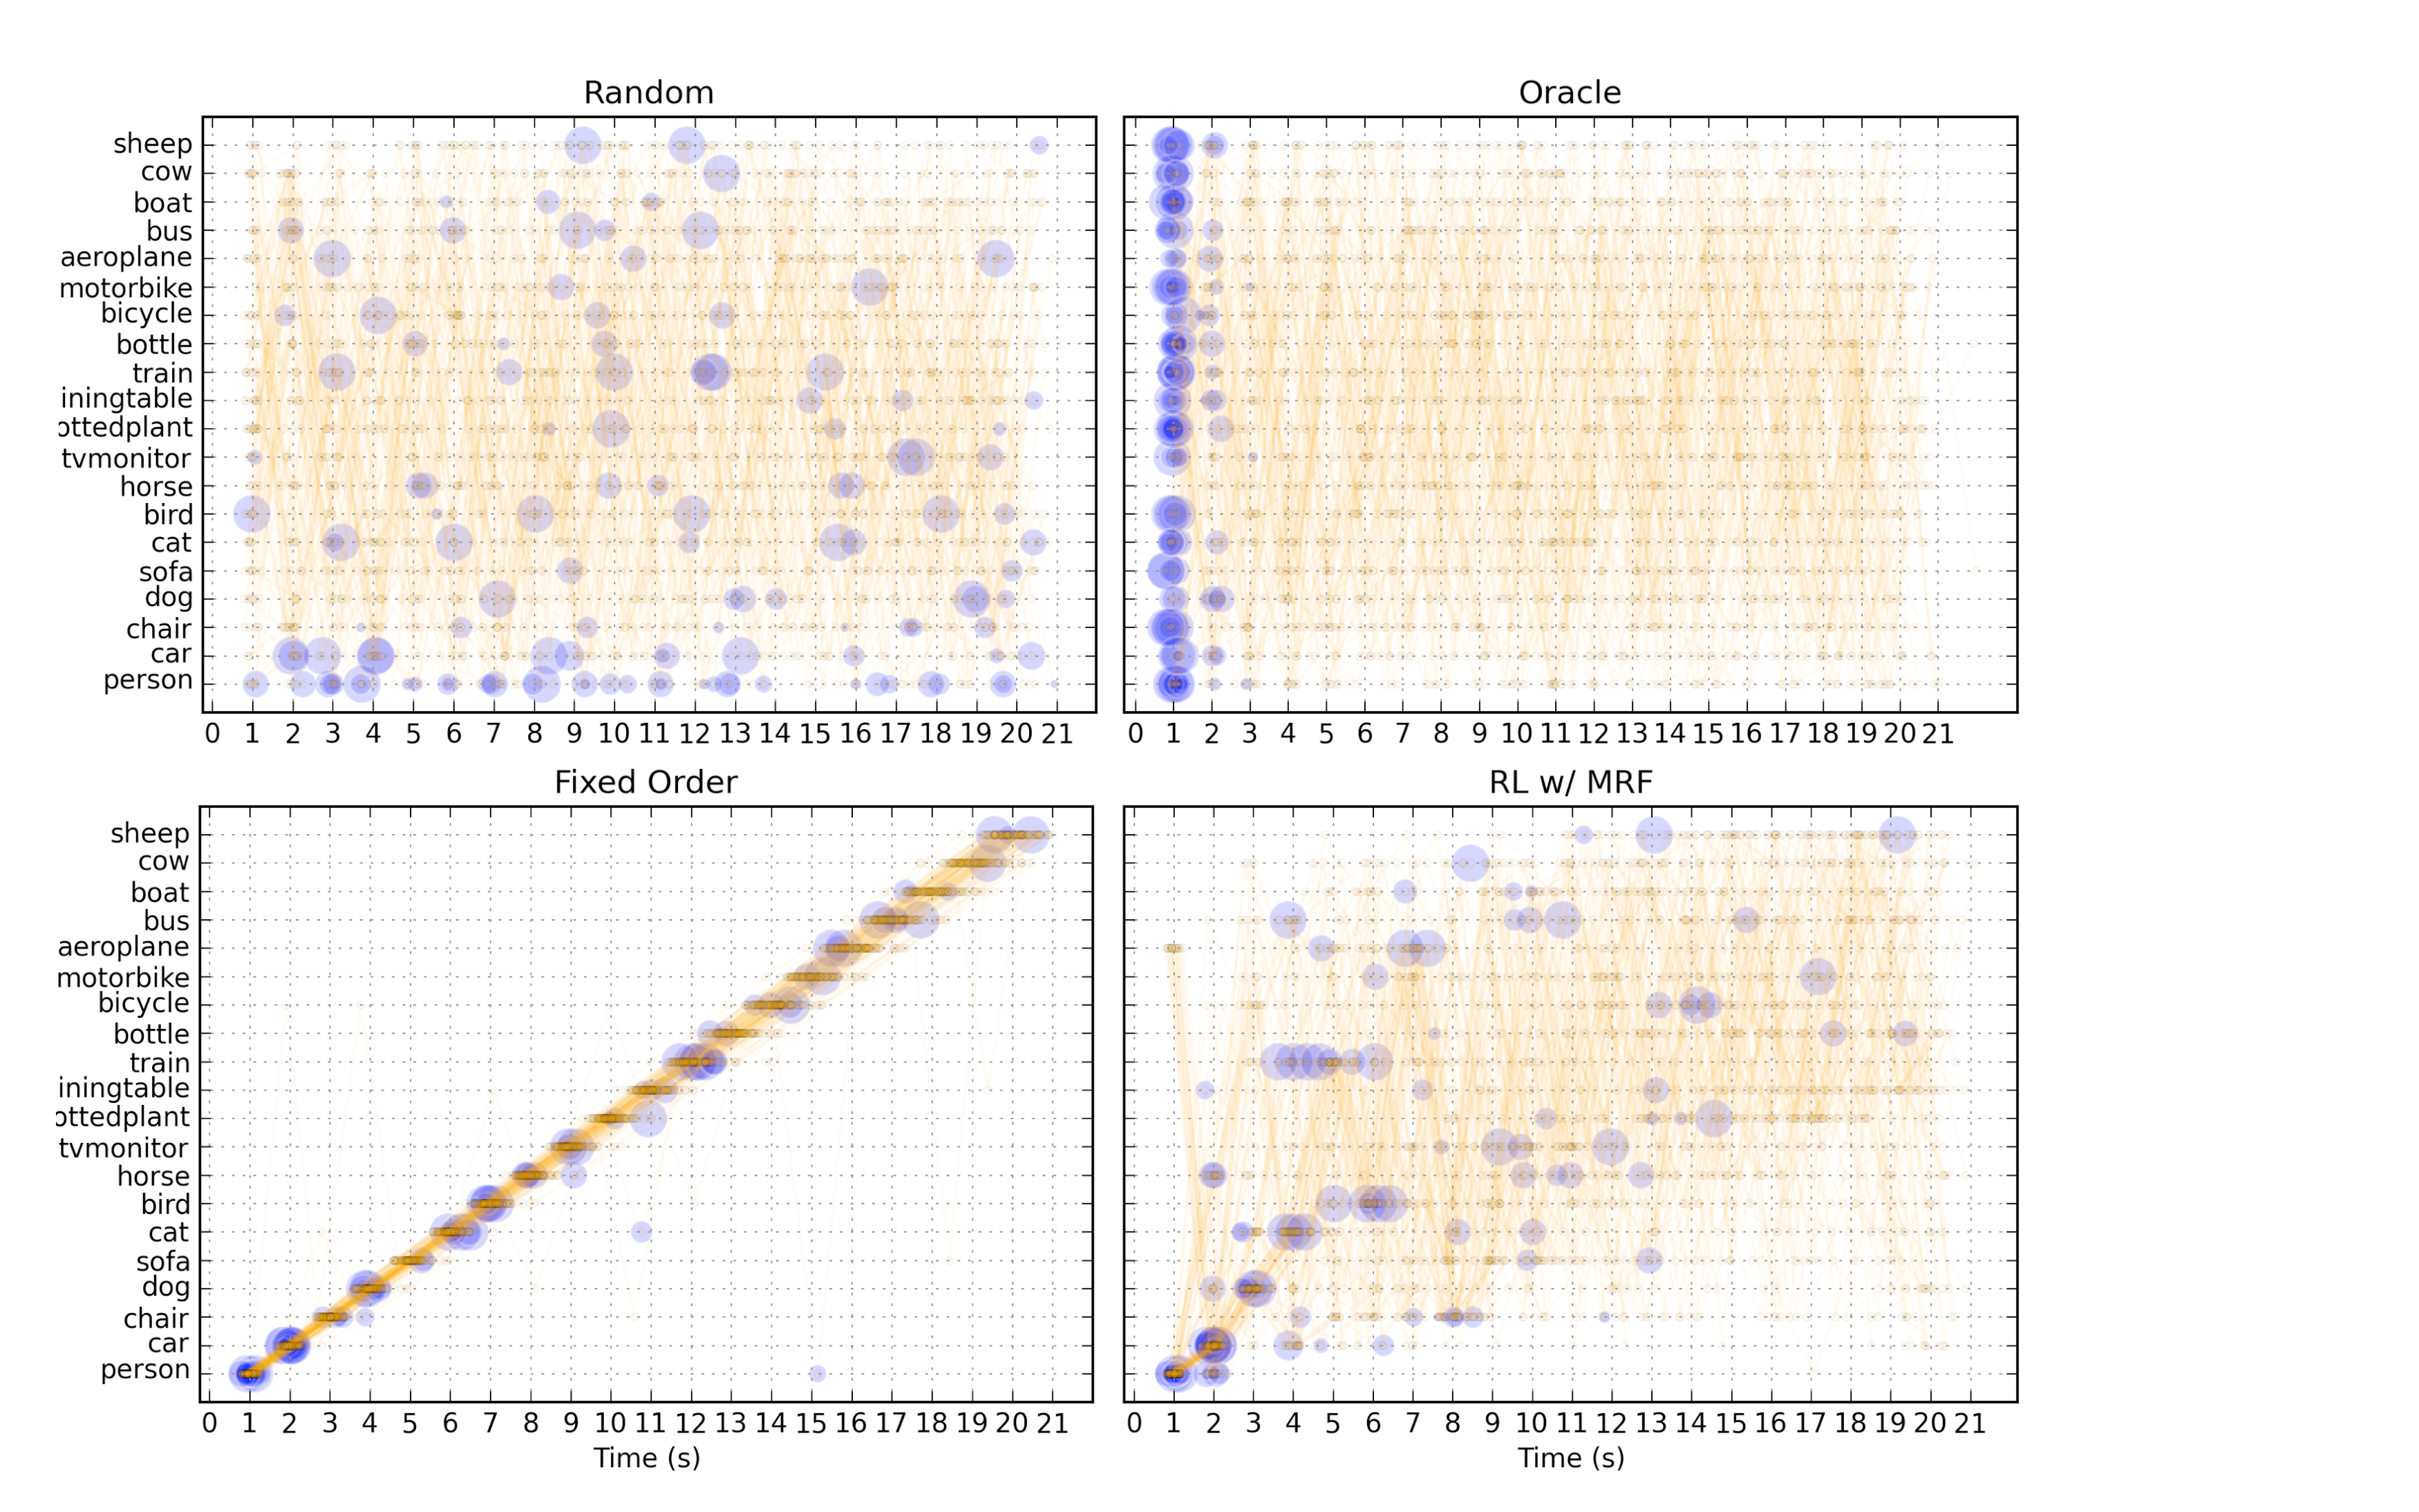
\includegraphics[width=\linewidth]{../../../2011-2012/figures/trajectories.pdf}
\caption[
Visualizing action trajectories of different object detection policies.]{
Visualizing the action trajectories of different policies.
Action selection traces are plotted in orange over many episodes; the size of the blue circles correspond to the increase in AP obtained by the action.
We see that the \textbf{Random} policy selects actions and obtains rewards randomly, while the \textbf{Oracle} policy obtains all rewards in the first few actions.
The \textbf{Fixed Order} policy selects actions in a static optimal order.
Our \textbf{RL w/ MRF} policy does not stick a static order but selects actions dynamically to maximize the rewards obtained early on.
}
\label{fig:trajectories}
\end{figure}
